\begin{itemize}
    \item Integration only with administration portal to be non invasive
    \item Only one connector for the administration portal
\end{itemize}

\begin{figure}[h]
    \centering
    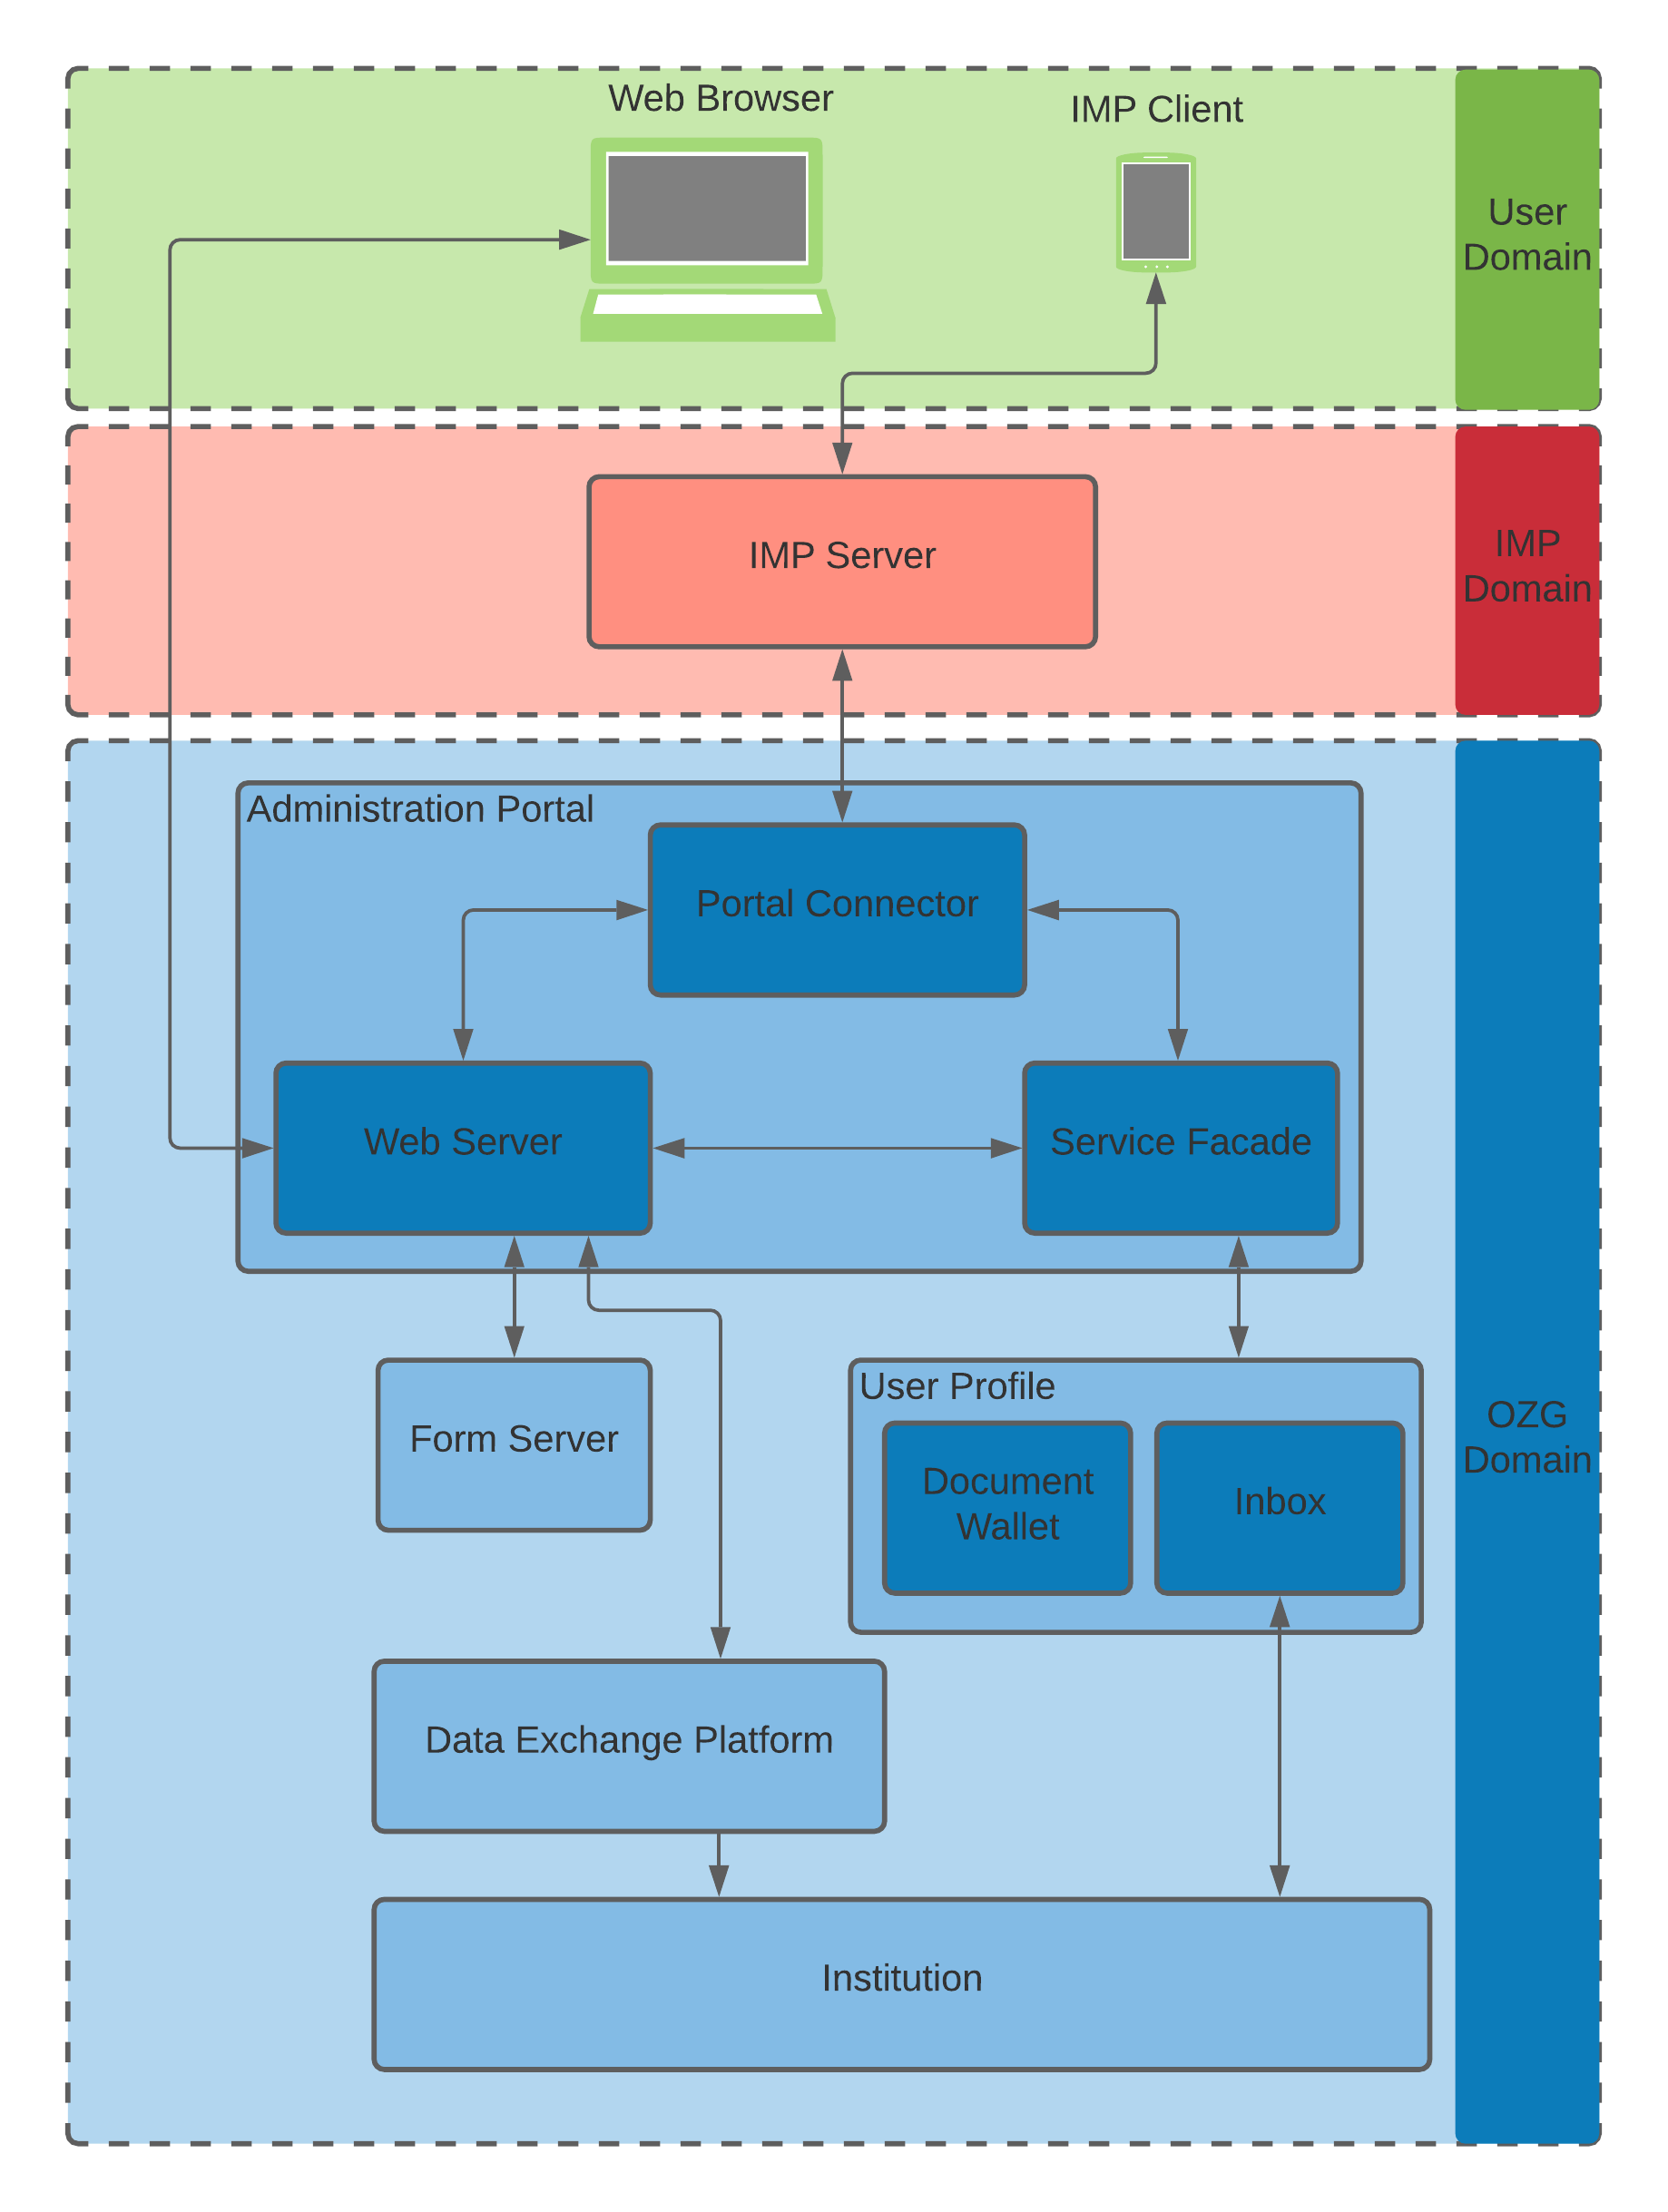
\includegraphics[scale=0.15]{Diagrams/Integration Architecture 1/Overview.png}
\end{figure}

\subsection{Messaging}

This section describes the advantages of using a message based integration approach.

...

\subsection{Modularity}

\begin{itemize}
    \item Use the Request-Reply methodology of the REST interface (only system sends requests, only connector sends replies) and expand it by a notification feature where only the connector sends notifications.
    \item Make Request-Reply functionality accessible to the messaging system through system request and connector reply modules.
    \item Make notification functionalities accessible to the messaging system through system notification and connector notification modules
    \item Solutions presented in the previous chapter rely on relationships and messages therefore make relationships and messages accessible to the messaging system through system relationship and system message modules. Those modules both rely on request and notification modules.
    \item To finally implement the features described in the previous chapter, multiple feature modules exist.
    \item All modules besides those for the connector can exist in multiple configurations: A feature module for example requires a system relationship module which is configured to only send and receive special types of relationships
    \item Examples
    \begin{itemize}
        \item Feature Module
        \begin{itemize}
            \item Attribute Change
            \item IMP Identity Connection
            \item Exchange mail
        \end{itemize}
        \item System Relationship Module
        \begin{itemize}
            \item Connection Relationship
            \item Administrative Service Application Relationship
        \end{itemize}
        \item System Request Module
        \begin{itemize}
            \item Create Template
            \item Send Relationship Response
        \end{itemize}
        \item System Message Module
        \begin{itemize}
            \item attribute change request
            \item incoming mail
        \end{itemize}
        \item System notification module
        \begin{itemize}
            \item new message
            \item relationship request
        \end{itemize}
    \end{itemize}
\end{itemize}

\begin{figure}[h]
    \centering
    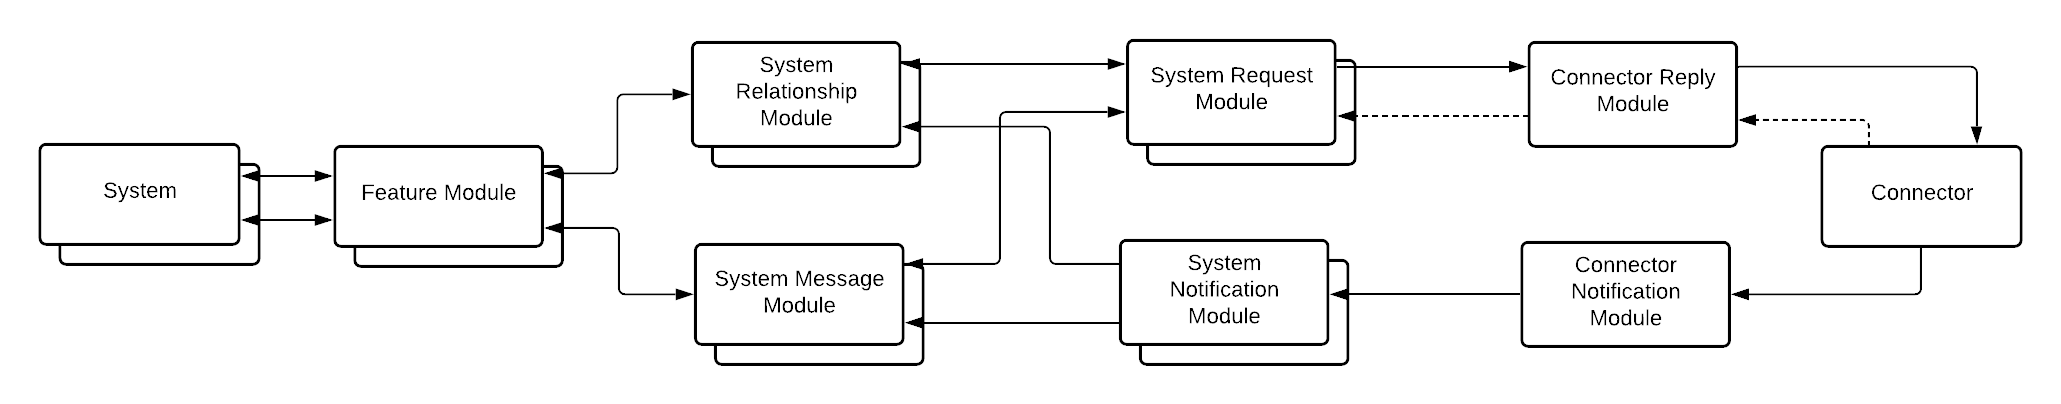
\includegraphics[scale=0.15]{Diagrams/Integration Architecture 1/Technological Integration/Connector/0. Modules Overview.png}
\end{figure}


\subsection{Connector Integration}

\begin{itemize}
    \item 
\end{itemize}

\begin{figure}[h]
    \centering
    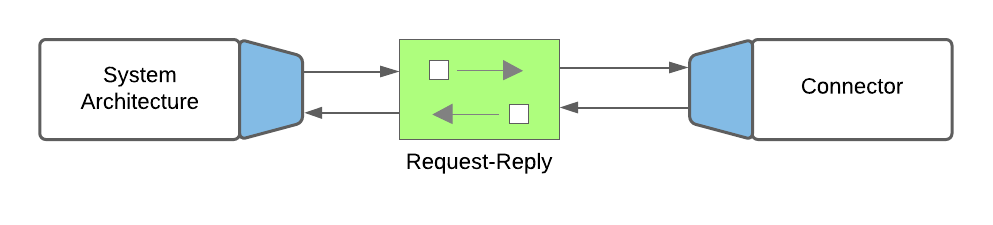
\includegraphics[scale=0.15]{Diagrams/Integration Architecture 1/Technological Integration/Connector/1. Request-Reply.png}
\end{figure}

\begin{figure}[h]
    \centering
    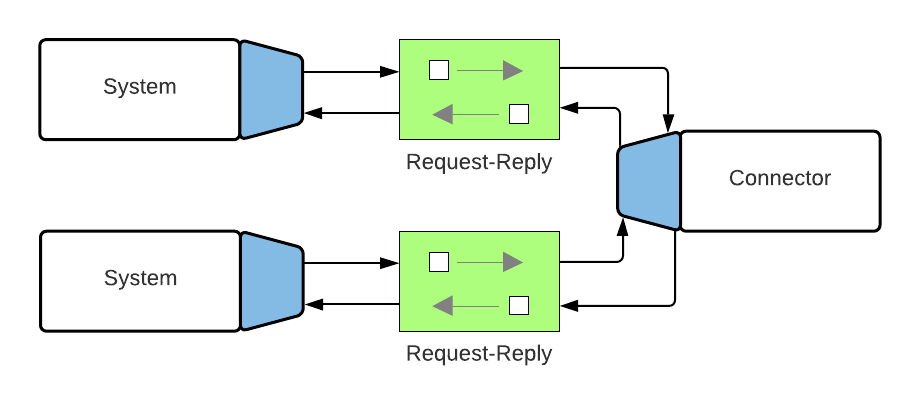
\includegraphics[scale=0.15]{Diagrams/Integration Architecture 1/Technological Integration/Connector/2. Multiple Systems.png}
\end{figure}

\begin{figure}[h]
    \centering
    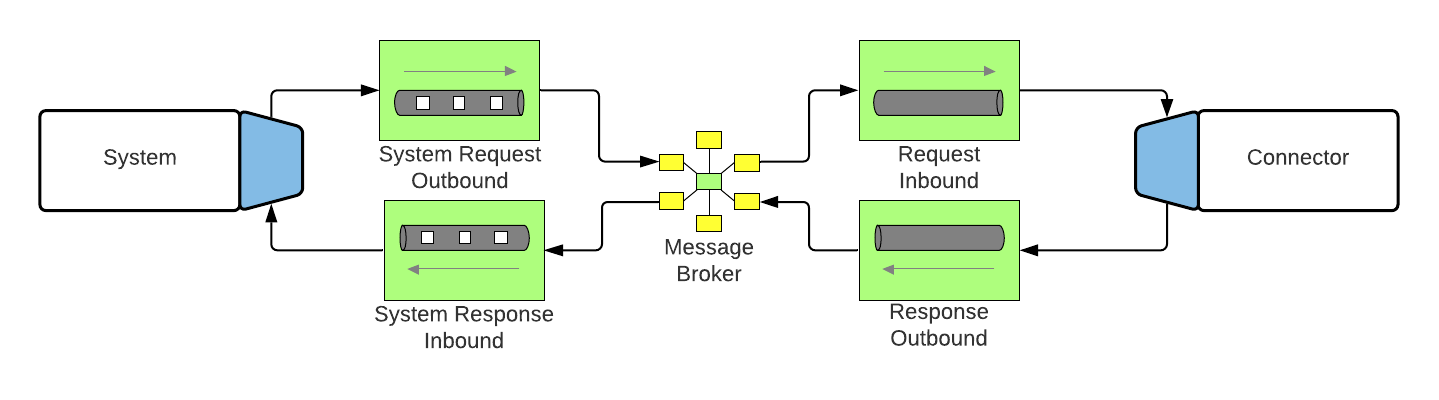
\includegraphics[scale=0.15]{Diagrams/Integration Architecture 1/Technological Integration/Connector/3. Routing.png}
\end{figure}

\begin{figure}[h]
    \centering
    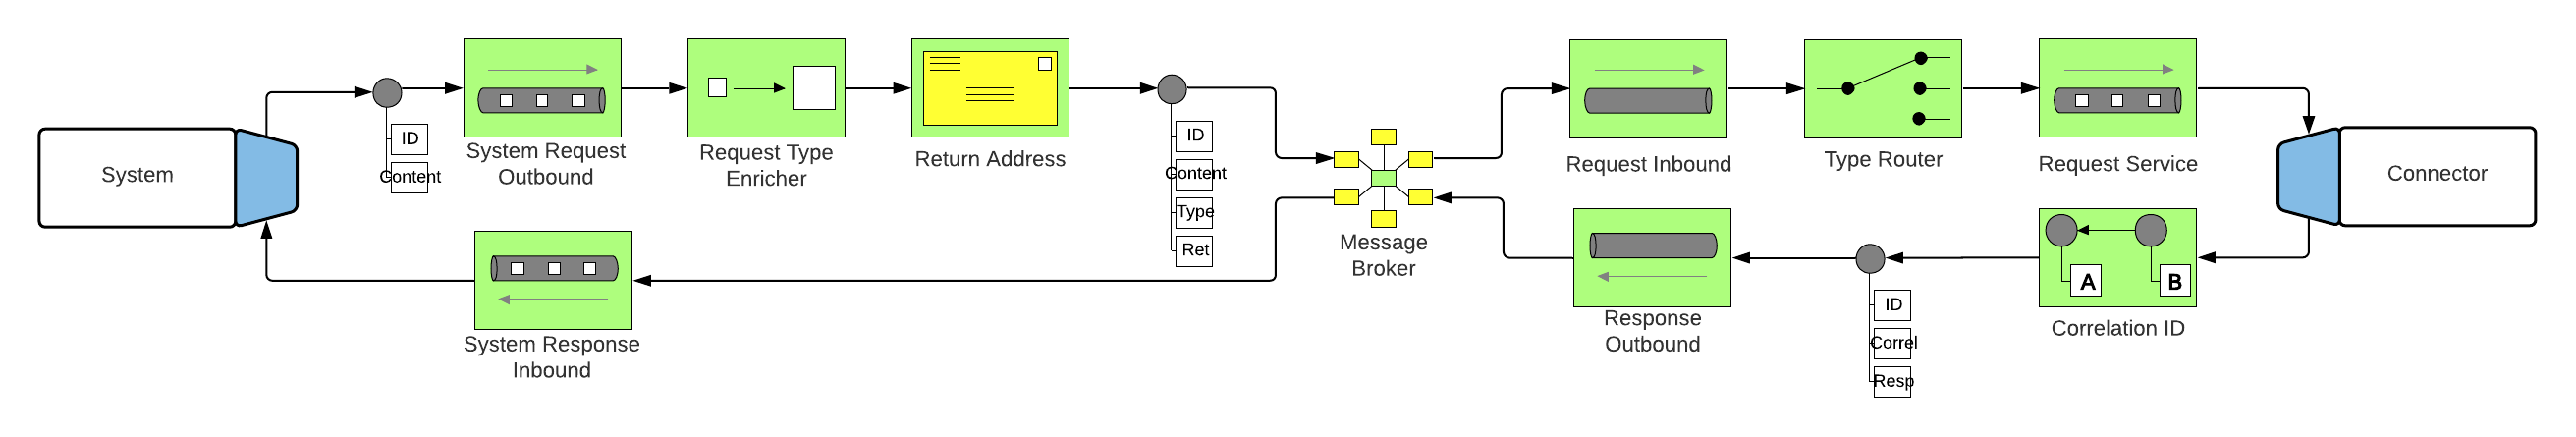
\includegraphics[scale=0.15]{Diagrams/Integration Architecture 1/Technological Integration/Connector/4. Routing Detail.png}
\end{figure}

\begin{figure}[h]
    \centering
    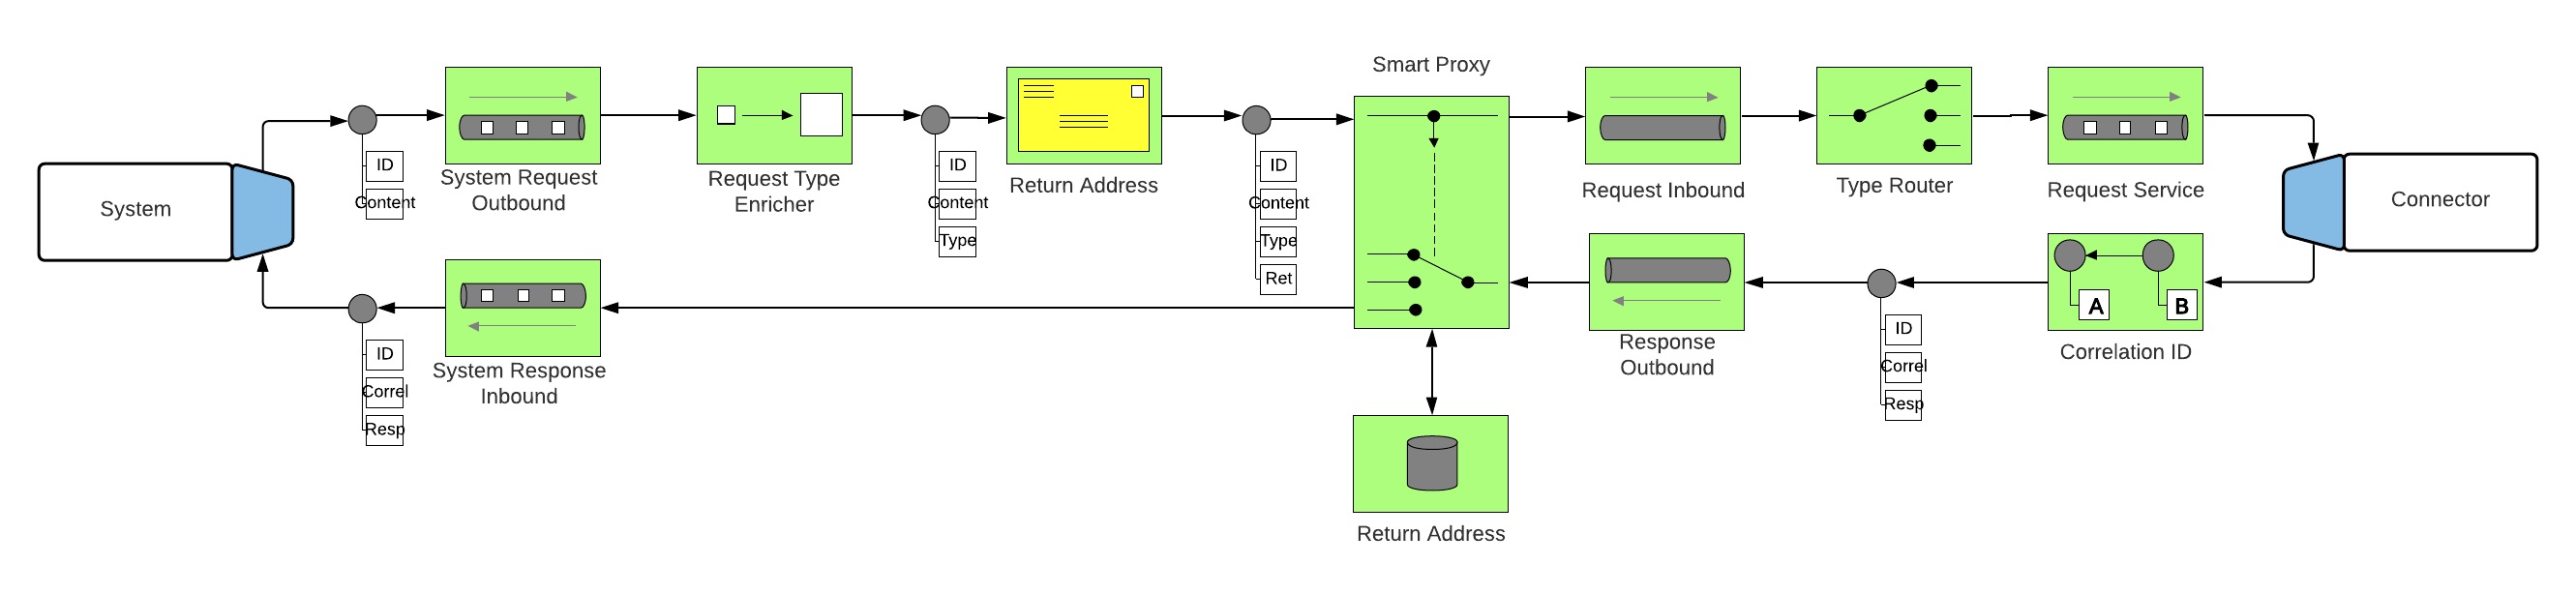
\includegraphics[scale=0.15]{Diagrams/Integration Architecture 1/Technological Integration/Connector/5. Proxy.png}
\end{figure}

\begin{figure}[h]
    \centering
    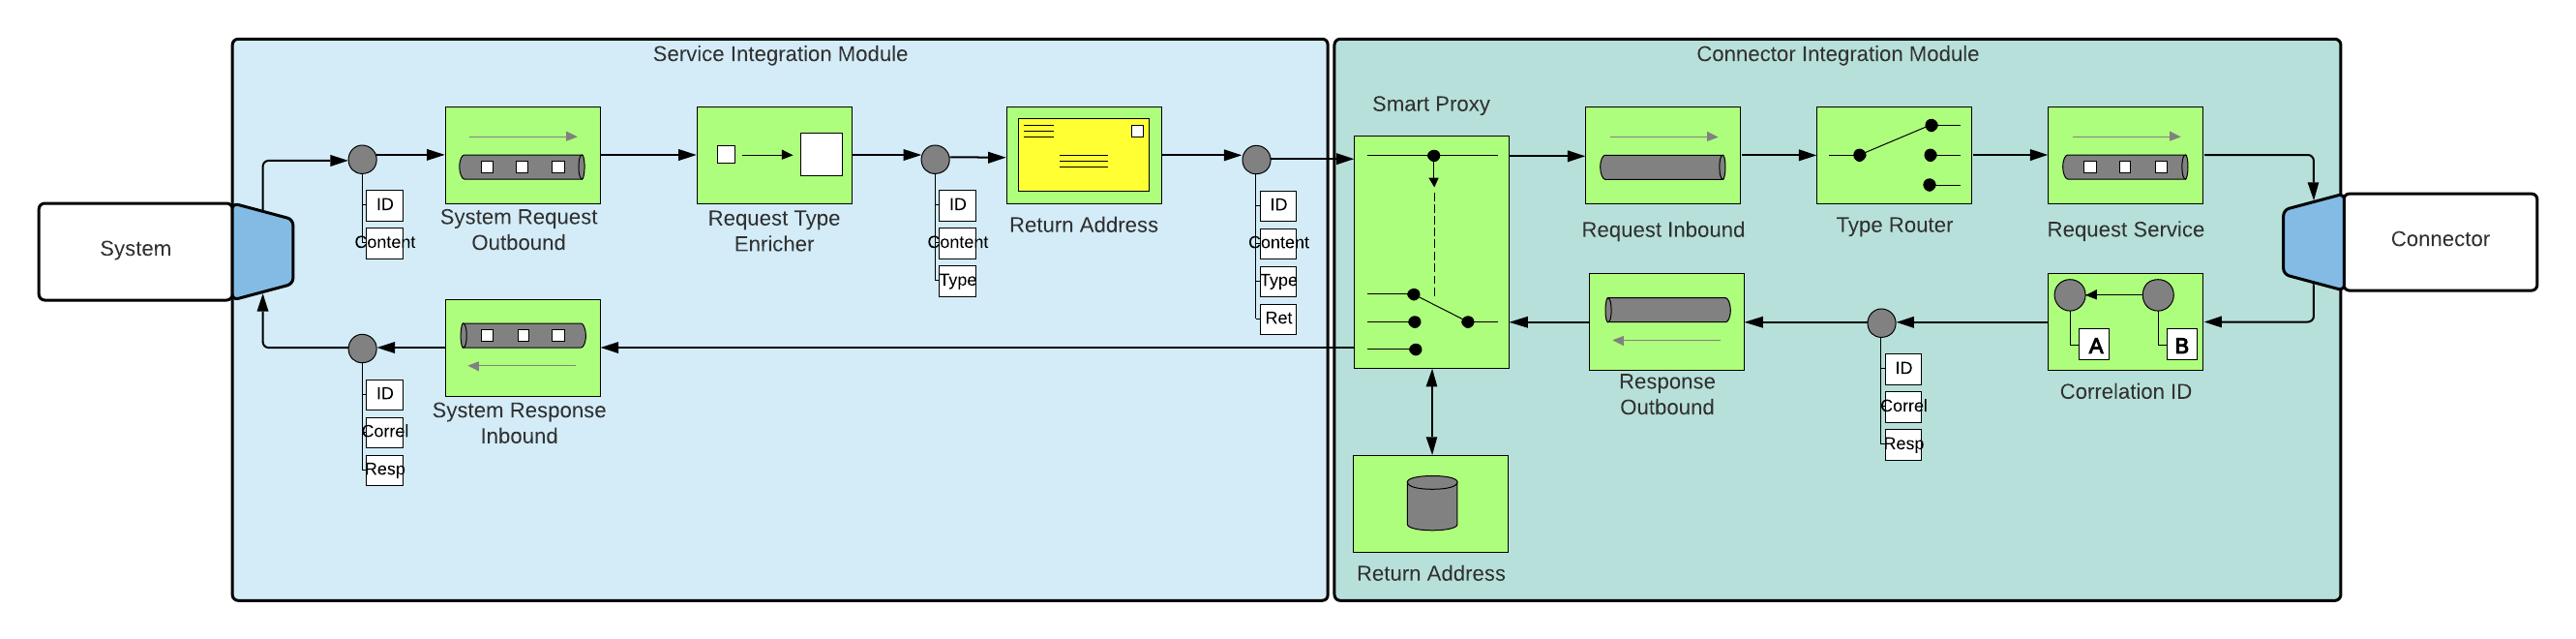
\includegraphics[scale=0.15]{Diagrams/Integration Architecture 1/Technological Integration/Connector/6. Integration Modules.png}
\end{figure}

\begin{figure}[h]
    \centering
    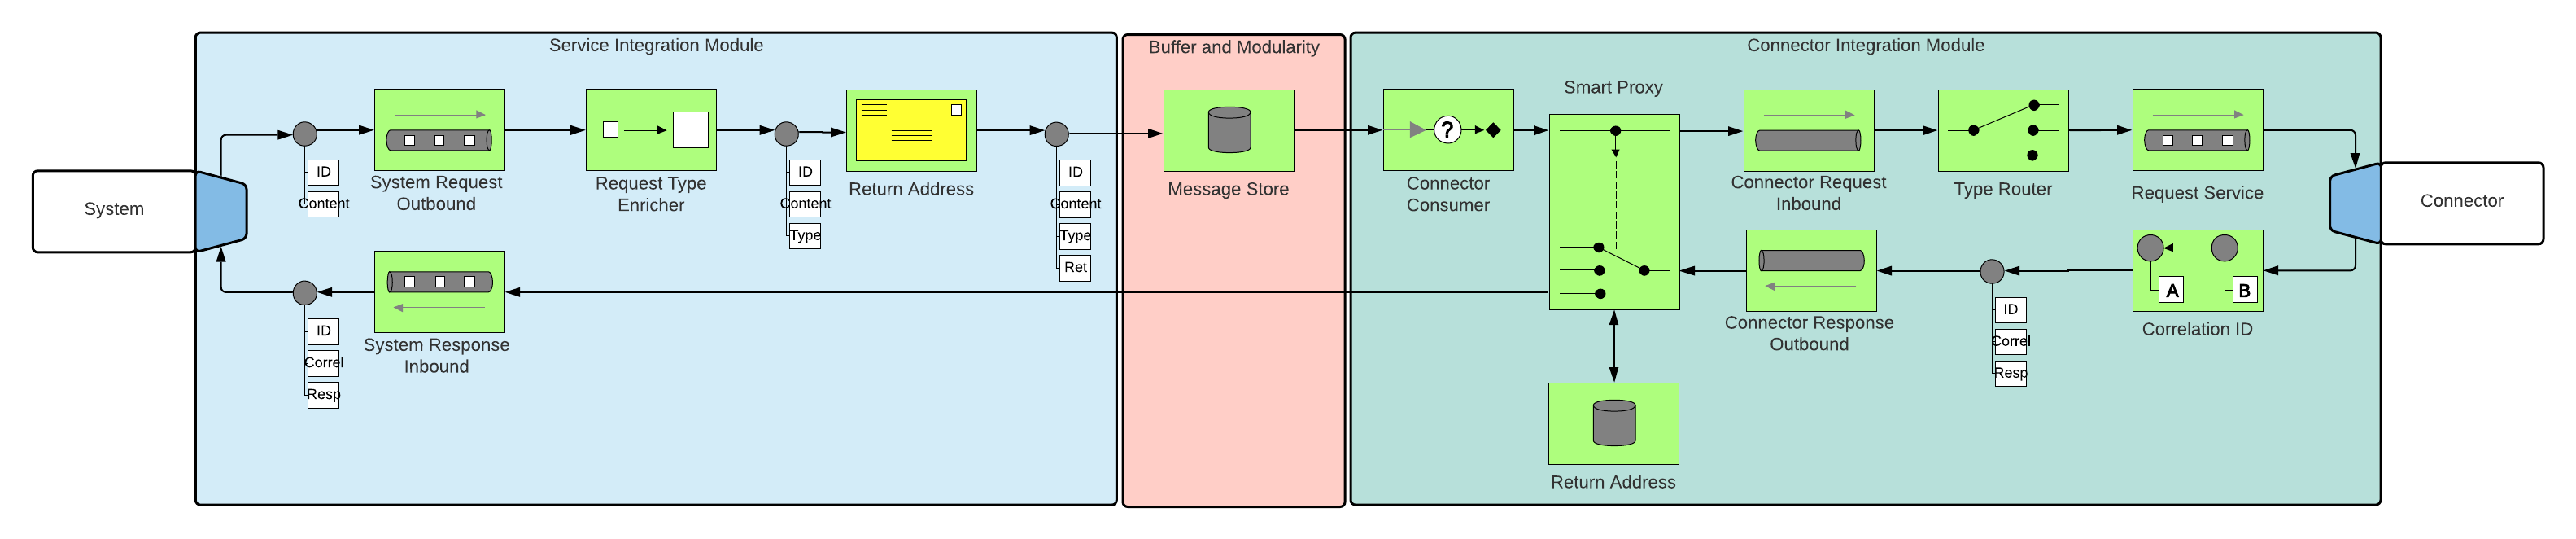
\includegraphics[scale=0.15]{Diagrams/Integration Architecture 1/Technological Integration/Connector/7. Buffer Modularity.png}
\end{figure}


\subsection{Relationship Integration}

\subsection{Message Integration}

\subsection{Attribute Mapping}
